
\chapter*{Introduction\markboth{\bf Introduction}{}}
\label{chap:intro}
\addcontentsline{toc}{chapter}{Introduction}

Inclusive electron scattering is a simple and powerful tool to probe the structure of the nucleus and Deep Inelastic Scattering (DIS) regime allows access to its partonic structure. The nucleus, itself can be used as a medium to study how nucleons and consequently partons are modified when embedded in the nuclear environment. The modification of quark and gluon distributions in bound nucleons was first realized through the modification of the per-nucleon cross sections of nucleons bound in nuclei, known as the "EMC effect".

For moderate Bjorken $x_B$, 0.35 $\leqslant$ $x_B$ $\leqslant$ 0.7, the per-nucleon DIS structure function for nuclei with A $\geqslant$ 3 was found to be suppressed compared to that of deuterium, leading to the phenomenon known as the ``EMC effect'' \cite{Aubert1983a, Ashman:1988bf, Arneodo:1988aa, Arneodo:1989sy, Gomez:1993ri, Allasia:1990nt, Seely2009}.

Since its discovery, the EMC effect has been a subject of extensive theoretical investigations aimed at understanding the underlying physics. While progress has been made in interpreting the main features of the effect, no single model has been able to explain the effect and its $x_B$ and $A$ \cite{Geesaman1995, Norton2003, Malace:2014uea} dependencies. A unifying understanding of the physical picture is still under intense debate. Most models of the EMC effect can be classified into two main categories:
%
\begin{itemize}
 \item ``Conventional'' nuclear models \cite{Ericson1983,Dunne1985,Akulinichev1985,Jung1988} in which the effect could be understood by a reduced effective nucleon mass in the nuclear potential, causing a shift of $x_B$ to higher values ($x_B$-rescaling or binding models). In these models the mass shift is often accompanied by an increased density of virtual pions associated with the nuclear force (pion cloud models). 
%
 \item Models involving the change of the quark confinement size in the nuclear medium \cite{Close1983,Nachtmann1984,Jaffe1984,Close1988} can be viewed, in the language of QCD, as Q$^2$ rescaling models. In some cases a simple increase of the nucleon radius is assumed (nucleon swelling), while in others quark deconfinement is invoked and the nucleon degrees of freedom are replaced by multi-quark clusters. 
\end{itemize}

\begin{figure}[tb]
  \begin{center}
     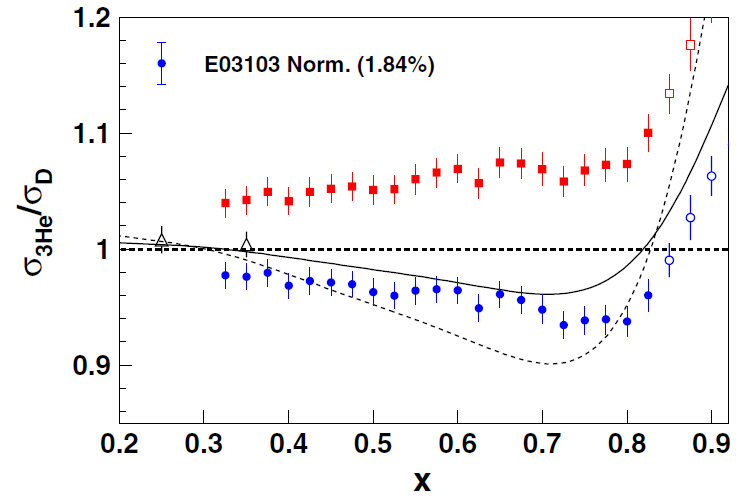
\includegraphics[angle=0, width=0.7\textwidth]{./fig-intro/seely_3he}
    \caption{EMC ratio $^3$He, the upper squares are the raw $^3$He/$^2$H ratios, while the bottom circles show the isoscalar EMC ratio. The triangles are the HERMES results~\cite{Ackerstaff2000} which use a different isoscalar correction. The solid (dashed) curves are the SLAC $A$-dependent fits to carbon and $^3$He~\cite{Seely2009}.}
    \label{fig:He3_hallc}
  \end{center}
\end{figure}

\begin{figure}[tb]
  \begin{center}
    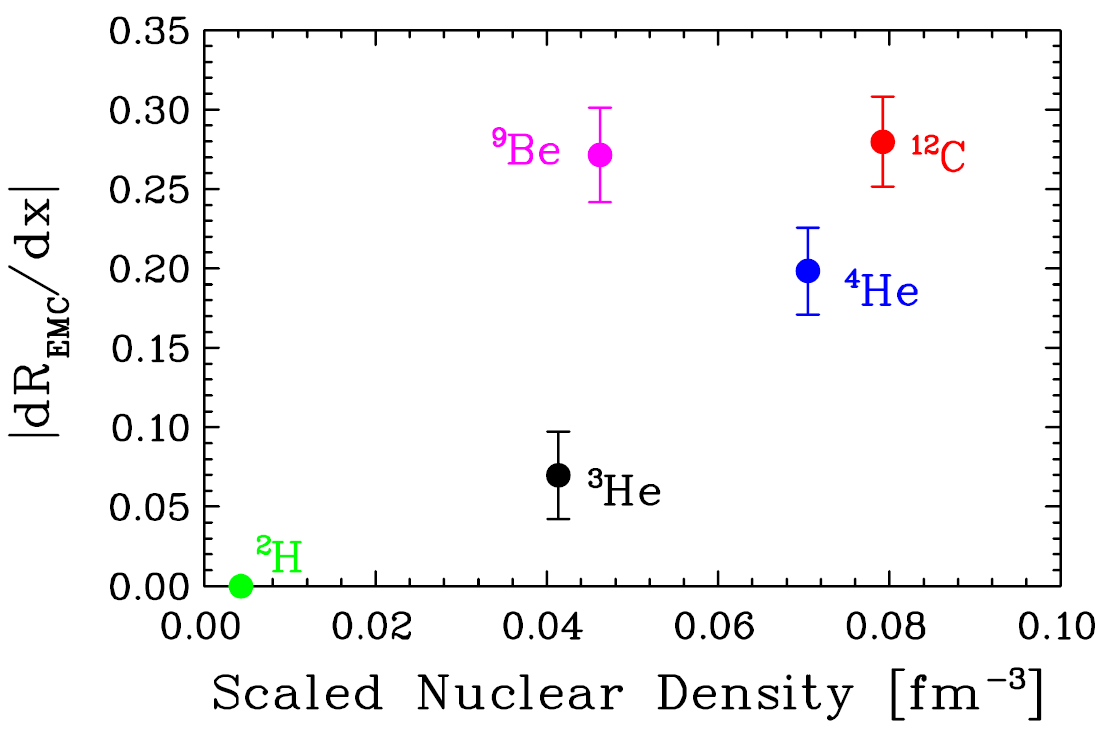
\includegraphics[angle=0, width=0.6\textwidth]{./fig-intro/seely_ratio}
    \caption{The slope of the isoscalar EMC ratio for $0.35<x_B<0.7$ as a function of nuclear density~\cite{Seely2009}.}
    \label{fig:ratio_hallc}
  \end{center}
\end{figure}

Recent experiment at Jefferson Lab measured the EMC effect for a series of light nuclei~\cite{Seely2009}. Fig.~\ref{fig:He3_hallc} shows the first measurements of the EMC effect for $^3$He at large $x_B$. It is found to be roughly one third of the effect observed in $^4$He, violating the $A$-dependent fit to the SLAC data, in the same way, the large EMC effect found in $^9$Be contradicts a simple density-dependent behavior (Fig.~\ref{fig:ratio_hallc}). This suggests that the EMC effect may be sensitive to the local density or details of the nuclear structure, some models have predicted this local EMC effect and describe the modification of the nucleons depending on their shells \cite{Kumano1990,ciofiliuti1991,CiofidegliAtti1999}. The possibility of the EMC effect depending on the local environment of the nucleon also motivates the investigation of possible connections between the EMC effect and other density-dependent effects such as short range correlations \cite{Higinbotham:2010ye, Weinstein:2010rt}.

\begin{figure}[tb]
  \begin{center}
    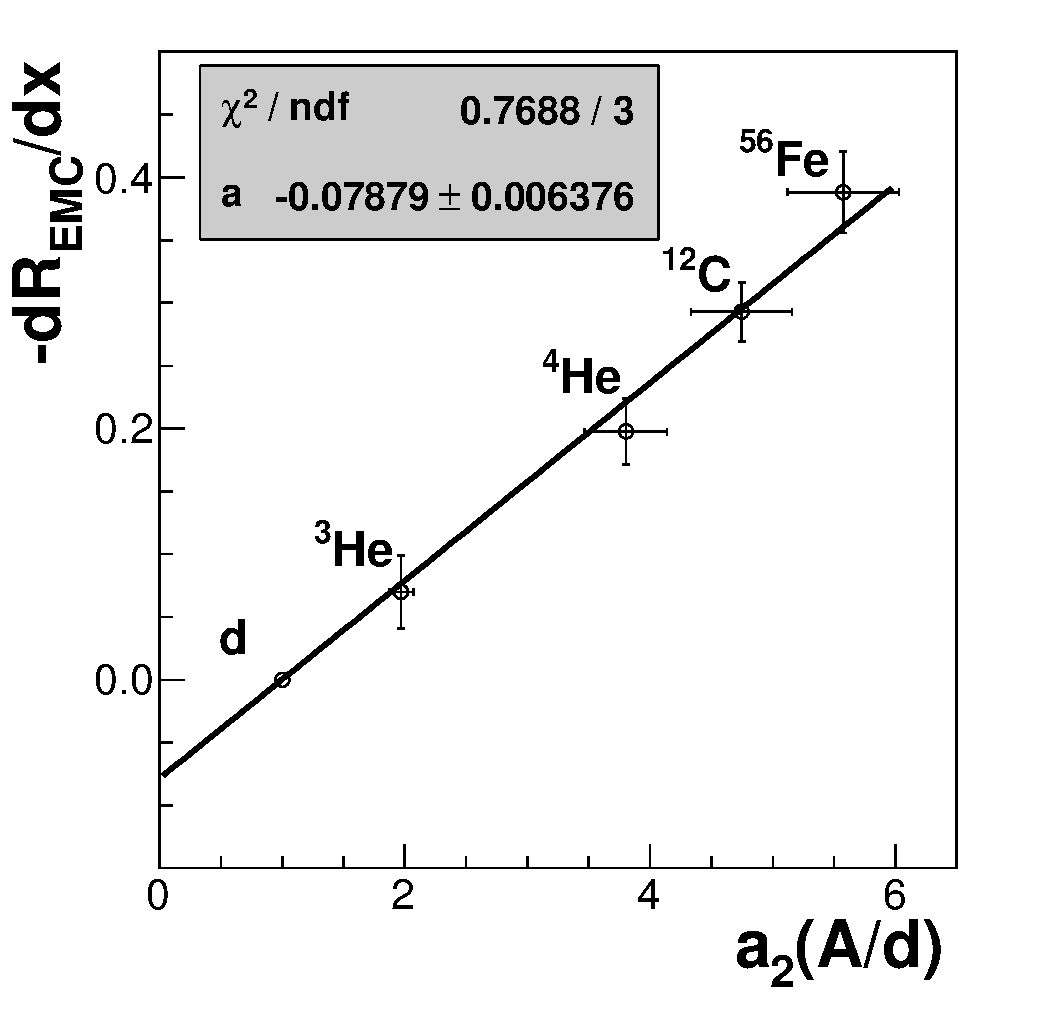
\includegraphics[angle=0, width=0.5\textwidth]{./fig-intro/Slope}
    \caption{The EMC slopes versus the SRC scale factors.  The uncertainties include both statistical and systematic errors added in quadrature.  The fit parameter is the intercept of the line and also the negative of the slope of the line.}
    \label{fig:src-emc}
  \end{center}
\end{figure}

Short range correlations (SRC) occur between nucleons located at less than the average inter-nucleon distance with high relative momentum \cite{Frankfurt:1993sp, Egiyan:2003vg, Egiyan:2005hs}. Those pairs of nucleons carry 80\% of all nucleons kinetic energy inside the nucleus although they only represent about 20\% of the nucleons. The probability for a nucleon to belong to a SRC pair is between 5\% in deuterium and about 20\% in nuclei such as carbon and iron.  The plateau obtained in the inclusive cross section ratios of two nuclei (for example iron and deuterium) in the region $x_B > 1.5$ for $Q^2 > 1.5$ GeV$^2$ indicates that for nucleon momentum larger than Fermi momentum ($p\geqslant p_{N} \simeq$ 275 MeV/c), the nucleon momentum distributions in different nuclei have similar shapes but differ in magnitude. The ratio of the cross sections in the plateau region also called the "SRC scale factor $a_{2N}(A/d)$" was found to be linearly correlated with the slope of the EMC effect \cite{Weinstein:2010rt}. This striking correlation shown in Fig.~\ref{fig:src-emc} could indicate that high momentum bound nucleons are important players in the EMC effect. To investigate the matter further, it is important to study the EMC effect as a function of both $x_B$ and the nucleon virtuality, by measuring the recoil fragment in addition to the scattered electron. 

